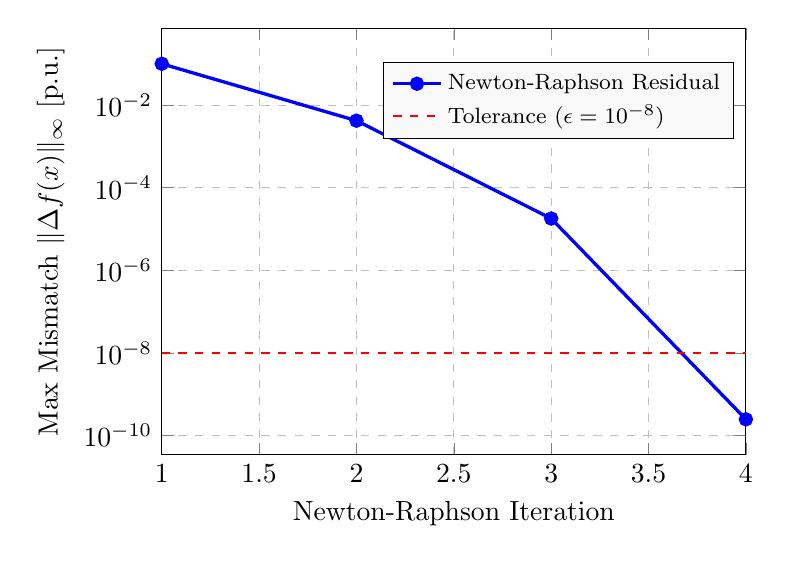
\begin{tikzpicture}
\begin{axis}[
    xlabel={Newton-Raphson Iteration},
    ylabel={Max Mismatch $\|\Delta f(x)\|_\infty$ [p.u.]},
    ymode=log,
    xmin=1, xmax=4,
    xmajorgrids,
    ymajorgrids,
    grid style=dashed,
    width=9cm,
    height=7cm,
    legend style={
        at={(0.98,0.92)},
        anchor=north east,
        font=\footnotesize,
        draw,
        fill=gray!5,
        legend cell align={left},
    },
]
  \addplot[color=Blue, mark=*, mark size=2pt, line width=1.2pt] coordinates {
    (1, 1.0000e-01)
    (2, 4.2000e-03)
    (3, 1.8000e-05)
    (4, 2.4885e-10)
  };
  \addlegendentry{Newton-Raphson Residual}
  \addplot[color=red, dashed, line width=1.0pt, domain=1:4] {1e-8};
  \addlegendentry{Tolerance ($\epsilon = 10^{-8}$)}
\end{axis}
\end{tikzpicture}